% CAST MANUAL LATEX
% This is the official manual for the CAST program package
\documentclass[10pt,a4paper]{article} %DOCUMENTCLASS

%%%% PACKAGES
\usepackage[utf8]{inputenc} %ENCODING
\usepackage[english]{babel} %ENGLISH LANGUAGE STYLE
\usepackage[parfill]{parskip} %PARAGRAPH SPACING
\usepackage{color} %COLOURS
\usepackage{tabularx} %BETTER TABLES THROUGH TABULARX
\usepackage{listings} %ENABLE (SOURCE) CODE LISTINGS
\usepackage{underscore} %AUTOMATICLY ESCAPING UNDERSCORES
\usepackage{graphicx} %LATEX CANT MANAGE IMAGES, SO WE NEED THIS
\usepackage{hyperref} %ENABLE URL SUPPORT
\usepackage[backend=bibtex,style=chem-angew,biblabel=dot]{biblatex} %REFERENCES
\addbibresource{castManualReferences.bib} %ADD BIBLATEX REFERENCES FILE.
\usepackage{acronym} %SUPPORT FOR ABBREVIATIONS


%%%%OPTIONS FOR CODE LISTINGS
\lstset{ %
	backgroundcolor=\color{white},   % choose the background color; you must add \usepackage{color} or \usepackage{xcolor}
	basicstyle=\footnotesize,        % the size of the fonts that are used for the code
	breakatwhitespace=false,         % sets if automatic breaks should only happen at whitespace
	breaklines=true,                 % sets automatic line breaking
	%captionpos=b,                    % sets the caption-position to bottom
	frame=single,	                 % adds a frame around the code
	keepspaces=true,                 % keeps spaces in text, useful for keeping indentation of code (possibly needs columns=flexible)
	%language=Octave,                 % the language of the code
	numbers=left,                    % where to put the line-numbers; possible values are (none, left, right)
	numbersep=5pt,                   % how far the line-numbers are from the code
	showspaces=false,                % show spaces everywhere adding particular underscores; it overrides 'showstringspaces'
	showstringspaces=false,          % underline spaces within strings only
	showtabs=false,                  % show tabs within strings adding particular underscores
	stepnumber=1,                    % the step between two line-numbers. If it's 1, each line will be numbered
	tabsize=2,	                     % sets default tabsize to 2 spaces
}

%%%%AUTHOR INFORMATION
\title{CAST Manual}
\author{Working Group Engels \\
	Julius-Maximilians Univeristy Wuerzburg \\
	Wuerzburg, Germany}

%%%%%%%%%%%%%%%%%%%%%%%%%%%%%%%%%%%%
%%%%                            %%%%
%%%%     CONDITIONALS           %%%%
%%%%                            %%%%
%%%%%%%%%%%%%%%%%%%%%%%%%%%%%%%%%%%%
% Different versions of the manual generatable through custom conditionals
\newif\ifverbose %VERBOSE
%VERBOSE: Use this conditional to describe procedures in detail or write detailed usage describtions which bloat the manual.

\newif\ifdevelopment %DEVELOPMENT
%DEVELOPMENT: Notes for people who have access to the CAST source and / or are coding inside CAST

\newif\ifdevmode %DEVMODE
%DEVMODE: Notes we (the authors of this manual) pass to each other.

\devmodetrue
\verbosetrue
\developmenttrue

\begin{document}
	\pagenumbering{Roman}
	%%%%%%%%%%%%%%%%%%%%%%%%%%%%%%%%%%%%
	%%%%                            %%%%
	%%%%     TITLE PAGE             %%%%
	%%%%                            %%%%
	%%%%%%%%%%%%%%%%%%%%%%%%%%%%%%%%%%%%

	% FRONT PAGE

	CAST - Conformational Search and Analysis Tool

	\ifdevelopment
		Manual for developers and programmers
	\else
		Manual
	\fi

	\ifverbose\else
		quick reference - short version
	\fi

	\ifdevmode
		\colorbox{red}{DEV MODE! THIS MANUAL IS NOT DESTINED TO BE RELEASED!}
	\fi

	Version 3.1 \\
	\today

	\ifdevmode
	\colorbox{red}{WE SHOULD REALLY PUT THE CAST ICON HERE!}
	\fi


	%%%%%%%%%%%%%%%%%%%%%%%%%%%%%%%%%%%%
	%%%%                            %%%%
	%%%%     TABLE OF CONTENTS      %%%%
	%%%%                            %%%%
	%%%%%%%%%%%%%%%%%%%%%%%%%%%%%%%%%%%%
	\newpage
	\tableofcontents

	%%%%%%%%%%%%%%%%%%%%%%%%%%%%%%%%%%%%
	%%%%                            %%%%
	%%%%     LIST OF FIGURES        %%%%
	%%%%                            %%%%
	%%%%%%%%%%%%%%%%%%%%%%%%%%%%%%%%%%%%

	\newpage
	\listoffigures

	%%%%%%%%%%%%%%%%%%%%%%%%%%%%%%%%%%%%
	%%%%                            %%%%
	%%%%     LIST OF TABLES         %%%%
	%%%%                            %%%%
	%%%%%%%%%%%%%%%%%%%%%%%%%%%%%%%%%%%%
	\newpage
	% We don't need this right now
	%\listoftables

	%%%%%%%%%%%%%%%%%%%%%%%%%%%%%%%%%%%%
	%%%%                            %%%%
	%%%%     LIST OF ABBREVIATIONS  %%%%
	%%%%                            %%%%
	%%%%%%%%%%%%%%%%%%%%%%%%%%%%%%%%%%%%
	\section{Table of Abbreviations}
	\begin{acronym}[DEINEMUDDA] % längste Abkürzung steht in eckigen Klammern
		\setlength{\itemsep}{-\parsep} % geringerer Zeilenabstand
		\acro{AMBER}{Assisted Model Building with Energy Refinement}
		\acro{CAST}{Conformational Analysis and Search Tool}
		\acro{CENCALC}{Conformational Entropy Calculations}
		\acro{DOF}{degree of freedom}
		\acrodefplural{DOF}[DOFs]{degrees of freedom}
		\acro{dRMSD}{distance root-mean-square deviation}
		\acro{GAFF}{General Amber Force Field}
		\acro{GPU}{graphics processing unit}
		\acro{MC}{Monte-Carlo}
		\acro{MCM}{Monte-Carlo with Minimization}
		\acro{MD}{Molecular Dynamics}
		\acro{NMR}{nuclear magnetic resonance}
		\acro{PCA}{Principal Component Analysis}
		\acro{PDF}{probability density function}
		\acro{PES}{potential energy surface}
		\acro{PMF}[PmF]{probability mass function}
		\acro{RMSD}{root-mean-square deviation}
		\acro{SVD}{singular value decomposition}
		\acro{TS}{TabuSearch}
		\acro{VMD}{Visual Molecular Dynamics}
	\end{acronym}
	\newpage

	%%%%%%%%%%%%%%%%%%%%%%%%%%%%%%%%%%%%
	%%%%                            %%%%
	%%%%     PREFACE                %%%%
	%%%%                            %%%%
	%%%%%%%%%%%%%%%%%%%%%%%%%%%%%%%%%%%%
	\pagenumbering{arabic}
	\section{Preface}
	The \ac{CAST} allows the accurate treatment of large and flexible (macro-)molecular systems. For the determination of thermally accessible minima \ac{CAST} offers the newly developed \ac{TS} algorithm\supercite{tabusearch}, as well as \ac{MC}\supercite{mc_original}, \ac{MCM} and molecular dynamics (MD) implemntations. For the determination of reaction paths CAST provides the PathOpt, the Nudged Elastic Band (NEB) and the Umbrella Sampling (US) approach. Access to free energies is possible through the free energy perturbation (FEP) approach. Along with a number of standard force fields, a newly developed Symmetry Adapted Perturbation Theory based force field (SAPT-FF) is included. Semi-empirical computations are possible through DFTB+ and MOPAC interfaces. For calculations based on Density Functional Theory (DFT), a MPI interface to the GPU accelerated TeraChem program is available. For more information on CAST see \cite{cast}.
	\newpage


	%%%%%%%%%%%%%%%%%%%%%%%%%%%%%%%%%%%%
	%%%%                            %%%%
	%%%%     COMPILING CAST         %%%%
	%%%%                            %%%%
	%%%%%%%%%%%%%%%%%%%%%%%%%%%%%%%%%%%%
	\ifdevmode
	\section{Compiling CAST}
	The CAST source code is not openly distributed. Currently, CAST has no external dependencies. Compilation was verified using Microsoft Visual Studio 2015 Update 1 on Windows 10 and GCC 5.3 on SuseLinux. A makefile for LINUX operating systems is part of the source code repository.
	\fi
	\newpage
	%%%%%%%%%%%%%%%%%%%%%%%%%%%%%%%%%%%%
	%%%%                            %%%%
	%%%%       Installation         %%%%
	%%%%                            %%%%
	%%%%%%%%%%%%%%%%%%%%%%%%%%%%%%%%%%%%

	\section{Installation}
	CAST is distributed as a precompiled executable for Linux and Windows. Currently CAST has no external dependencies.

	\ifdevmode
		{Original text:

			2.1	Windows

		The Windows binary can be used with any Windows operating system starting from Windows 7. No further requirements exist.
		2.2	Linux
		Precompiled binaries are statically linked. FFTW 3.4 libraries have to be set in the PATH variable of the Linux shell.
		\textbf{LD\_LIBRARY\_PATH \glqq Path to FFTW lib dir\grqq}
	\fi
	\newpage

	%%%%%%%%%%%%%%%%%%%%%%%%%%%%%%%%%%%%%%
	%%%%                              %%%%
	%%%% General Structure and Useage %%%%
	%%%%                              %%%%
	%%%%%%%%%%%%%%%%%%%%%%%%%%%%%%%%%%%%%%
	\section{General Structure and Usage}
	CAST features several main computation methods which can be combined with force fields, semi-empirical or DFT methods via several interfaces. Input file formatting and available commands are discussed in the following paragraphs.



	%%%% Inputfile %%%%
	\subsection{Inputfile}
	A file named \glqq CAST.txt\grqq or \glqq INPUTFILE\grqq can be used to change the configuration options of CAST. It may contain CAST option keywords followed by one or more appropriate values. The keywords are case sensitive. Comments can be included by starting the line with a \#. The variables are usually of type integer, floating point or boolean.\\

	The following input commands are compulsory for CAST to work and have to be set for every calculation.\\~\\
	\begin{tabularx}{\textwidth}{l|l|l}
		Variable&	Effect &	Default \\
		\hline
		verbosity &	Amount of CAST output &	1\\
		cores &	Number of OpenMP threads &	1\\
		name &	Name of input file &	none\\
		outname &	Name of output files &	none\\
		input-type &	Format of coordinate file &	TINKER\\
	\end{tabularx}\\~\\

	The keyword for the path of the used coordinate file is "name". The variable “cores” controls the number of threads if CAST has been compiled with OpenMP\supercite{openmp08}. “outname” defines the name of the outputfile with information regarding the calculation.
	The switch controlling how much information CAST will print to the console is named "verbosity". Proper values are positive integral numbers where low numbers indicate less in-formation than higher numbers do. Suitable values for productive use are 1, 2 or 3.



	 An example input for a single point calculation with the OPLS-AA force field is given below:

	\colorbox{red}{NOTE: INSERT SAMPLE INPUTFILE HERE}


	%%%% Force Fields %%%%
	\subsection{Force fields}
	CAST features four different force field implementations in the code. The \textbf{OPLS-AA}\supercite{oplsaa, oplsaa2}, \textbf{CHARMM}\supercite{charmm}, \textbf{AMBER}\supercite{amber} and \textbf{AMOEBA}\supercite{amoeba} force fields. With the exception of the AMOEBA force field, the non-bonded parts of the force fields have been parallelized using the OpenMP programming model. Furthermore, the FEP and SPME methods can only be used with OPLS-AA, CHARMM and AMBER at the moment.
		%% AMOEBA and short range correction
		\subsubsection{AMOEBA and short range correction}
		\ifdevmode \colorbox{red}{Blalala yaddayaddayadda… insert stuff here.} \fi
		%% Smooth particle Mesh Ewald
		\subsubsection{Smooth particle Mesh Ewald}
		The smooth particle mesh ewald\supercite{spme} allows the treatment of full electrostatic in periodic sys-tems. Essential for the use of the SPME are applied periodic boundary conditions The SPME uses the FFTW 3.4 library for the fourier transformations of the charge grid $($see Installation details$)$.  SPME control features the following parameters:\\~\\

		\begin{tabularx}{\textwidth}{l|l|l}
			variable & effect & default \\
			\hline
			PME & Switches pme on or off 0 = off, 1 = on & 0 \\
			PMEspline & Spline order used in SPME & 5 \\
			PMEtreshold & Affects the value of the ewald coefficient & 0.00000001 \\
		\end{tabularx}

	%%%% Energy Interfaces %%%%
	\subsection{Energy Interfaces}
	The energy interfaces are the main parts of CAST for the choice of the underlying computational method. Via the interface the different force fields can be accessed as well as the interfaces to external programs. For semi-empirical calculations an interface to MOPAC2012 (serial\supercite{mopac} and parallel\supercite{mopac_parallel}) is present, for DFT computations the GPU accelerated program Tera-Chem can be accessed. Both programs are not part of the CAST distribution and the authors are not responsible for access to those programs. MOPAC is freely available from the MOPAC website. TeraChem\supercite{terachem} can be purchased at the PetaChem website.
	The following interfaces and keywords are available:\\~\\
	\begin{tabularx}{\textwidth}{l|l|l}
		Interface & Type & Further input \\
		\hline
		\textbf{OPLS-AA} & internal & parameterfile \\
		\textbf{AMBER} & internal & parameterfile \\
		\textbf{CHARMM22} & internal & parameterfile \\
		\textbf{AMOEBA} & internal & parameterfile\\
		\textbf{SAPT-FF} & internal &parameterfile and Spackman-input\\
		\textbf{MOPAC} & external & MOPAC variables\\
		\textbf{TeraChem} & external & TeraChem input\\
	\end{tabularx}	\\~\\
	In contrast to the force fields the MOPAC and TeraChem interfaces do not need correct force field parameters to function. Only the coordinate file has to be in TINKER format but can be generated with arbitrary parameters.
		%% MOPAC
		\subsubsection{MOPAC}
		MOPAC is accessed via system call. The MOPAC interface expects the MOPAC executable path to be either \glqq \textbackslash opt\textbackslash mopac\textbackslash MOPAC2012.exe\grqq on linux or \glqq C:\textbackslash Program Files\textbackslash mopac\textbackslash MOPAC2012.exe\grqq on Windows systems by default. The path can be changed using \glqq MOPACpath\grqq.
		The keywords, handed over to MOPAC and controlling the calculation can be adjusted via the \glqq MOPACkey\grqq \ $($default \glqq PM7 MOZYM\grqq$)$ parameter.
		If the value of the keyword \glqq MOPACdelete\grqq \ $($default 1$)$ is set to 0, CAST will not delete the temporary in- and output transfer-files written by CAST or MOPAC.

		\begin{tabularx}{\textwidth}{l|l|l}
			variable & effect & default \\
			\hline
			MOPACkey & Input parameters, see MOPAC manual & none\\
			MOPACpath & Path to MOAPC executable & none\\
			MOPACversion & Version of MOPAC (2007, 2012) & MOPAC2012\\
			MOPACdelete & Delete MOPAC temporary files 0=no, 1=yes & 0\\

		\end{tabularx}

		%% TeraChem
		\subsubsection{TeraChem}
		TeraChem\supercite{terachem} is accessed via MPI\supercite{mpi} interface and the keyword TERACHEM in the energy inter-face. All further parameters regarding basis set, functional and so on have to be set in an extra file readable by CAST. CAST then transfers the input parameters to TeraChem via the MPI interface. The syntax for the TeraChem input is such that each string needs to be set in its own line. Otherwise it’s identical to the TeraChem input. An example is shown in the fol-lowing. The name for the TeraChem input has to be \textit{CAST_TERACHEM_OPTIONS.txt}.

		\begin{lstlisting}
		basis
		cc-pvdz
		charge
		0
		method
		b3lyp
		dftgrid
		2
		dftd
		d2
		\end{lstlisting}

		Example of a TeraChem input readable by CAST. Each TeraChem option needs to be set in its own line.


	%%%% COORDINATES FILE %%%%
	\subsection{Coordinates file}
	CAST makes use of the TINKER style xyz file. This format has the advantage of carrying more information in the file than the standard xyz format. Programs that are able to read and/or write TINKER style files are Molden, VMD, Avogadro, Chem BioOffice, TINKER, Open Babel and some others. \\~\\
	A Tinker format file contains a sequence of structures where the first line of each structure contains the number of atoms while the following lines cover one atom each. The next table explicates the composition of the atom lines.\\~\\
	\ifverbose
	\begin{tabularx}{\textwidth}{l|l|l|l}
		Column & Width & Justification & Miscellaneous\\
		\hline

		\textbf{Number}	& 6			& R	& ~\\
		\textbf{\textit{Free}}	& 2			&  ~ & ~\\
		\textbf{Symbol}	& 3			& L	& ~\\
		\textbf{X coordinate in Å}	& 12			& R & 6 decimal places\\
		\textbf{Y coordinate in Å}	& 12			 & R & 6 decimal places\\
		\textbf{Z coordinate in Å}	& 12			& R	& 6 decimal places\\
		\textbf{Atomtype}	& 6			& R	& ~\\
		\textbf{Bound atoms}	& 6 (each index)			& R	& multiple values\\
	\end{tabularx}

	\textbf{Note}: For alchemical transformations during free energy perturbation simulations, each line may also contain the \glqq IN\grqq or \glqq OUT\grqq $($ case insensitive $)$ keyword at the end, separated by at least one space from the last bound atom.
	\fi

	%%%% TASKS %%%%
	\subsection{TASKS}
	All input information for CAST are put into a single input file. The name of the input file has to be either INPUTFILE $($case sensitive$)$ or CAST.txt. CAST also features command line parameters. The main computations in CAST are called \textit{tasks}. They are invoked with the keyword task followed by the name of the computation.

	\newpage

	%%%%%%%%%%%%%%%%%%%%%%%%%%%%%%%%%%%%%%
	%%%%                              %%%%
	%%%%     Specific Tasks           %%%%
	%%%%                              %%%%
	%%%%%%%%%%%%%%%%%%%%%%%%%%%%%%%%%%%%%%
	\section{Specific Tasks}

	%%%% SP %%%%
	\subsection{SP - Single point energy calculation}
	A single point calculation calculates the potential energy of the respective system Single points can be run with either force field or semi empirical or DFT calculations. In case of force field calculations the output is decomposed into the different force field contributions.\\

	The output consists of the abbreviations for the different force field contributions as well as their respective energy in $\frac{kcal}{mol}$. At the end the total potential energy is given in $\frac{kcal}{mol}$.\\~\\

	\begin{tabularx}{\textwidth}{l|l}
		symbol & energy\\
		\hline
		\textbf{B} & Bond energy\\
		\textbf{A} & Angle energy\\
		\textbf{U} & Urey-Bradley energy (CHARMM\supercite{charmm})\\
		\textbf{ID} & Improper dihedrals energy (AMBER, CHARMM)\\
		\textbf{IT} & Improper torsions energy (OPLS-AA)\\
		\textbf{V} & Van-der-Waals energy\\
		\textbf{C} & Charge energy\\
		\textbf{SOLV} & Solvent energy (if implicit solvent is used)\\
		\textbf{SUM} & Total potential energy\\

	\end{tabularx}\\~\\


	%%%% GRAD %%%%
	\subsection{GRAD - Single point energy and gradient calculation}
	The result of a gradient calculation is the same as the result for a single point with the addi-tion that the gradients on the atoms are also calculated. The output is expanded of a file where the filename is extended by the keyword GRAD. This file contains the breakdown of the gradients with respect to atoms, force field contributions and x-, y- and z-coordinates.

	%%%% LOCOPT %%%%
	\subsection{LOCOPT - Local optimization}
	CAST is using the L-BFGS algorithm with the More and Thuente linesearch for local optimizations if an interface without optimizer is used or additional forces are applied.
	If an interface with included optimizer $($MOPAC, TeraChem, Tinker$)$ is used $($and if no bias forces are to be applied$)$, the optimization process will be carried out by those programs and CAST will only retrieve the final geometry and gradient values.
	The integrated L-BFGS can be adjusted regarding the maximum number of steps performed in the optimization routine via the "BFGSmaxstep"\ option $($default "10000"$)$.
	The convergence criterion can be altered using "BFGSgrad" $($default "0.001"$)$.

	\begin{tabularx}{\textwidth}{l|l|l}
		variable & effect & default \\
		\hline
		\textbf{BGFSgrad (float)} & Threshold for gradients & 0.0001 \\
		\textbf{BFGSmaxstep (integer)} & Number of max BFGS steps & 10000 \\
	\end{tabularx}

	%%%% MD %%%%
	\subsection{MD - Molecular Dynamics}
	The MD keyword is used to start a molecular dynamics calculation. MDs can be performed in NVE, NVT and NPT ensembles. For temperature control a Nose-Hoover thermostat is available. Pressure can be controlled by a Berendsen-barostat. If constant pressure is de-sired, the use of periodic boundary conditions is compulsory. Integration of the equations of motion can be done via a velocity-verlet or Beeman integration scheme.
	The following variables are used to control the molecular dynamics part of CAST:\\~\\

	\begin{tabularx}{\textwidth}{l|X|X}
		variable & effect & default \\
		\hline
		\textbf{MDsteps} & Number of MD steps & 0 \\
		\textbf{MDintegrator} & Type of integrator 0  = Velocity-verlet;	1  = Beeman integrator
		& 0 \\
		\textbf{MDveloscale} & Remove translation and rotation at every step 0 = no, 1 = yes & 0 \\
		\ifdevmode
		~ & \colorbox{red}{how does MDvelosclae work? we should describe this here} & ~ \\
		\fi
		\textbf{MDthermostat} & Constant temperature 0 = no, 1 = yes
		 & 0 \\
		\textbf{MDtimestep} & Timestep in picoseconds & 0.001 \\
		\textbf{MDtrack} & Track MD and write output 0 = no, 1 = yes & 0 \\
		\textbf{MDsnap} & Number of snapshots & x \ifdevmode \colorbox{red}{wtf is x?} \fi \\
		\textbf{MDsnap_buffer} & Number of snapshots saved in memory before written to file & x \ifdevmode \colorbox{red}{wtf is x?} \fi \\
		\textbf{MDsnap_opt} & Optimize snapshots 0 = no, 1 = yes & 0 \\
		\textbf{MDheat} (2 values) & 1st value: snapshot number; 2nd value: temperature at snapshot & 0 0.0\\
		\textbf{MDpress} & Enable pressure control 0 = no, 1 = yes & 0 \\
		\textbf{MDcompress} & compressibility of the solvent & 0.000046 (water) \\
		\textbf{MDpdelay} & Barostat delay in picoseconds & 2 \\
		\textbf{MDptarget} & Target pressure in atm & 1 \\
		\textbf{MDspehrical} (7 values) & Switch for spherical boundary conditions & 0 \ifdevmode \colorbox{red}{wtf, 7 values? clarify this plz} \fi \\
		\textbf{MDrattle} & Switch for H-bond constraints 0 = no, 1 = all hydrogen bonds & 0 \\
		\textbf{MDrattpar} & Parameter file for equilibrium distances of h-bonds & none \ifdevmode \colorbox{red}{uhm, is this variable a filename? if yes, clarify} \fi \\
		\textbf{MDrestart_offset} & Offset for restart file writing \ifdevmode \colorbox{red}{in frames? or picosec?}& 0 \\
		\textbf{MDrefine_offset} & Offset for nonbonded list generation & 0 \ifdevmode \colorbox{red}{wtf is this, clarify} \fi \\
		\textbf{MD_resume} & Boolean switch for using a restart file to start MD & 0 \\
	\end{tabularx}\\~\\

	\ifverbose
	Note: The settings for MDheat can be applied multiple times. The first number indicates the snapshot number, the second one the desired temperature at this snapshot. During the heat-ing process the thermostat is disabled and a simple velocity scaling is used to heat the sys-tem. If the MDheat keyword is applied multiple times heating and cooling can be applied sequentially during a single simulation. The program reads the MDheat keywords from top to bottom and starting with the one and top and finishing with the one on the bottom:\\~\\
	\begin{lstlisting}
	MDheat			    0  	  0.0
	MDheat 			 1000   300.0
	MDheat			 5000   300.0
	MDheat			10000     0.0
	\end{lstlisting}~\\~\\
	In the above example the simulation starts at 0 Kelvin and is heated to 300K within the first 1000 steps. The temperature is kept for 4000 steps until 5000 steps are reached. After that the system is cooled back to 0 Kelvin during steps 5000 to 10000. The user has to take care that enough total steps are performed for the temperature scaling sequence!
	\ifdevmode The settings for spherical boundary conditions are further discussed in section \colorbox{red}{XX}. \fi
	\fi

	%%%% UMBRELLA %%%%
	\subsection{UMBRELLA - Umbrella Sampling}
	The Umbrella sampling implementation features three reaction coordinates which can be sampled: distances, angles and dihedral angles. Distances can be chosen between any two particles in the system. Angles and dihedrals can be defined between any three or four par-ticles in the system. None of the reaction coordinates is limited to existing internal coordi-nates of the system.
	The umbrella sampling is divided into two parts: equilibration with the applied bias potential and production run with the applied bias potential. For all reaction coordinates a half har-monic potential is used. The number of steps for equilibration is defined by the USequil vari-able. The number of production steps is defined by the MDsteps variable.

	\begin{tabularx}{\textwidth}{l|X|X}
		variable & effect & default \\
		\hline
		\textbf{USequil} & number of equilibration steps & 0 \\
		\textbf{USsnap} & Offset for snapshots (Snapshot every x steps) & 0 \\
		\textbf{UStorsion} (6 values) & Definition for torsion angle & none \\
		\textbf{USdist} (4 values) & Definition for distance & none \\
	\end{tabularx}

	\ifverbose
	\textbf{\textit{UStorsion and USdist}}\\
	The syntax for the restraints definition can be seen in the following listing:\\

	\begin{lstlisting}
	#Torsion restraint    <atom 1> <atom 2> <atom 3> <atom 4> <force> <value>
	UStorsion                  1      5        7         9      0.05    0.0
	#Distance restraint   <atom 1> <atom 2> <force> <value>
	USdist                     1      9        10.0    3.0
	\end{lstlisting}
	~\\~\\
	Torsion restraints consist of 6 values: the first 4 integers are the index numbers of the atoms which form the dihedral. The fifth number is the force constant of the harmonic potential in $\frac{kcal}{deg^2}$ and the last index the desired value of the angle in degree.
	The distance restraint consist of the two indices for the atoms, the force constant in $\frac{kcal}{Å^2}$ and the distance in Å.
	The umbrella sampling output is written to the file "umbrella.txt". The output is written for use with the WHAM program for post processing. For details on the use of WHAM we refer the reader to the corresponding WHAM manual.
	\ifdevmode
	\colorbox{red}{wtf is wham? insert source or link or something}
	\fi
	\fi

	%%%% Free energy perturbation %%%%
	\subsection{FEP - Free energy perturbation}
	Free energy perturbation allows the alchemical transformation of one moiety into another and the derivation of the free energy change corresponding to the transformation. For FEP calculations the coordinate file has to be modified. CAST uses the dual topology paradigm to define the topology for the chimeric system. In the dual topology both states of the trans-formation are present during the simulation. Therefore, the input structure of the starting system has to be extended by the moiety of the final structure. As an example the transformation of ethane to ethane is shown: \\~\\

	\begin{figure}[h]
		\centering
		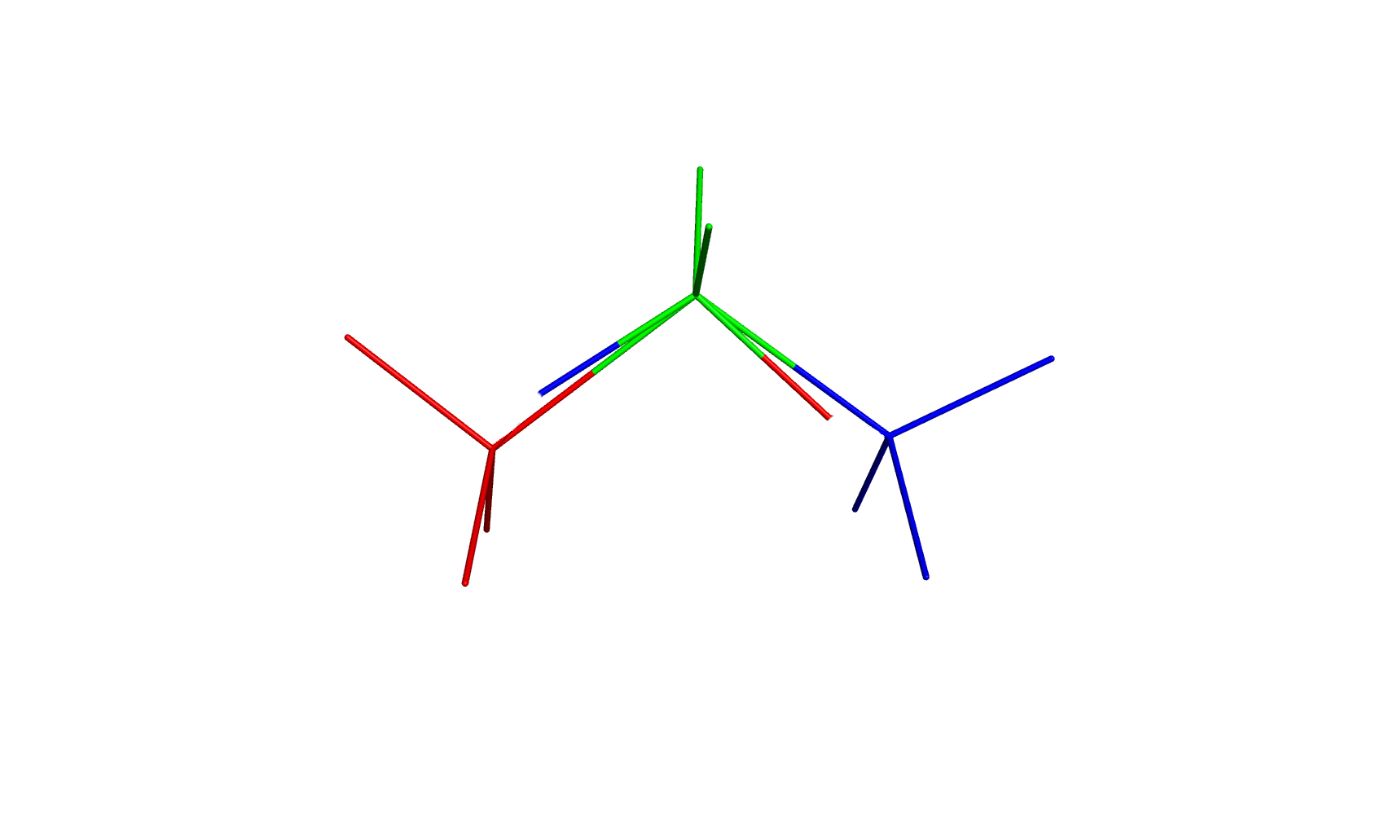
\includegraphics[width=0.5\textwidth]{img/imgfep1.png}
		\caption{Exemplifying FEP calculations in CAST}
		\label{fig:FEP1}
	\end{figure}
	The original Ethane is modified by adding another CH3-group + H to one of the ends of the methane. In the next step the atoms belonging to both the starting and the final stet have to be identified. They are marked in green in the picture. Those atoms don’t need to be modified in the input file and are always present in the simulation. The atoms marked in blue are the one belonging to the starting system and are phased “out” during the simulation. All at-oms belonging only to the starting point have to be marked with an IN in the coordinate file after the bonding partners. The atoms belonging to the final state of the system have to be marked with an OUT after the bonding partners. The modified file is shown in the following:\\~\\
	\begin{figure}[h]
		\centering
		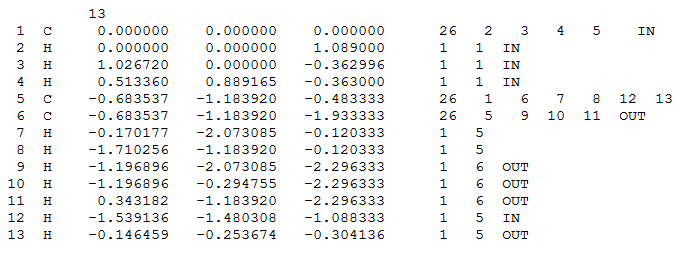
\includegraphics[width=0.95\textwidth]{img/imgfep2.png}
		\caption{Modifies tinker input style for FEP calculations}
		\label{fig:FEP2}
	\end{figure}
	One condition of the dual topology paradigm is that the atoms only belonging to start and end point must not interact with each other during the calculation. CAST takes care of this automatically by excluding all angles, dihedrals or non bonded interactions involving atom belonging to IN and OUT.
	FEP calculations can be modified with various parameters.

	\begin{tabularx}{\textwidth}{l|X|X}
		variable & effect & default \\
		\hline
		\textbf{FEPlambda} & Final value for order pa-rameter. Doesn’t need to be changed at all \ifdevmode \colorbox{red}{then why is it changeable? reconsider plz!} \fi & 1.0 \\
		\textbf{FEPdlambda} & Lambda increment. Lamb-da/Dlambda = number of FEP windows	& 0.05 \\
		\textbf{FEPvdwcouple} & Controls coupling of vdW interactions (see XX) \ifdevmode \colorbox{red}{what is XX? see where?} \fi & 1.0 \\
		\textbf{FEPeleccouple} & Controls coupling of electrostatics
		& 0.5 \\
		\textbf{FEPvshift} & Value for the vdw shifting parameter in the softcore potential & 4.0 \\
		\textbf{FEPcshift} & Value for shifting parameter in the electrostatic potential (not in use currently) \ifdevmode \colorbox{red}{if its not used, should we get rid of it?} \fi & 0.0 \\
		\textbf{FEPequil} & Number of equilibration steps in each window & none \\
		\textbf{FEPsteps} & Number of production steps in each window &  none\\
		\textbf{FEPfreq} & Frequency of FEP output & none \\
	\end{tabularx}\\~\\
	\ifdevmode \colorbox{red}{is the default behavior of FEPfreq reasonable? no output? reconsider plz}

	FEP calculations produce two output files: alchemical.txt and FEP_Results.txt. Alchemical contains detailed information about electrostatic and van-der-Waals interactions for the current lambda value. Furthermore, the current temperature and free energy change is dis-played. The file FEP_Results contains the total free energy change for the simulation and for each window.
	The FEP implementation is part of the MD code. Thermostats, barostats boundary conditions and all other parameters needed can be controlled with the MD variables.

	%%%% Dimer Method (DIMER) %%%%
	\subsection{DIMER - Dimer Method}
	The "dimer size" (magnitude of dimer vector) in the dimer method [Heyden, Bell; JChemPhys 123; 2005] can be controlled via "DIMERdistance" (default "0.01").
	It is possible to adjust the maximum rotational force during the dimer translation. The dimer translation is interrupted and the dimer is rotated into the minimum in case this limit is ex-ceeded. The key controlling this value is called "DIMERtflimit" (default "0.01").
	The maximum number of iterations for the dimer rotation and translation steps can be set in the combined "DIMERmaxit" option, which takes two parameters where the first one limits the number of rotation iterations per translation step while the second one represents the maximum number of translations (default value: "20 100", maximum number of total dimer iterations is therefore ).
	The convergence criterion for the dimer rotation (the angle that needs to be undercut) in degrees can be adjusted using "DIMERrotconvergence" (default: "5.0").

	\begin{tabularx}{\textwidth}{l|X|X}
		variable & effect & default \\
		\hline
		\textbf{DIMERdistance} & Controls magnitude of dimer vector & 0.01 \\
		\textbf{DIMERtflimit} & Controls magnitude of dimer force & 0.01 \\
		\textbf{DIMERmaxit} (2 values) & Controls rotation steps per translation and total translation steps & 20 100 \\
		\textbf{DIMERrotconvergence} & Convergence criterium for rotation in degree & 5.0 \\
	\end{tabularx}

	%%%% Global Optimization (GO) %%%%
	\subsection{GO - Global Optimization}
	The total number of steps for the global optimization routines is set by "Iterations" (default "1000"). Cast will save all minima between E_0 (current lowest energy) and $E_0 + D$ where the value of D is adjusted with the "Erange" keyword (default "0.0").
	If the current step does not result in a newly accepted minimum, CAST will select a new starting point. The key "GOfallback" selects either a simple fallback to local / global minimum (value "LAST_GLOBAL", default) or an evolutionary selection algorithm (value "EVOLUTION").

	\begin{tabularx}{\textwidth}{l|X|X}
		variable & effect & default \\
		\hline
		\textbf{Iterations} & Number of iterations & 1000 \\
		\textbf{Erange} & Energy range for output & 0.0 \\
		\textbf{GOfallback} & Type of fallback & LAST_GLOBAL \\
	\end{tabularx}

	%% Starting point selection
	\subsubsection{Starting point selection}
	\textbf{Simple Fallback} \\
	This method uses the parameter "GOfallback_limit" to determine how often the program can use a specific minimum as a starting point. If the limit for the last accepted minimum is reached, CAST uses the current "global" minimum instead. If the limit for this minimum has also been reached, CAST stops.\\~\\

	%% Evolutionary selection
	\textbf{Evolutionary selection} \\
	This algorithm selects a new starting point among a limited number of minima N. (The limit is set via "GOincluded_minima" and defaults to 10.)
	A roulette selection algorithm is applied where the fitness of the respective structures is de-termined based on their energetic rank. A lower L and an upper bound H for the fitness can be specified using "GOfitness_bounds" (default "0.5 1.0") where minimum N has fitness L and minimum 1 has fitness H.
	The interpolation between those points (1,H) -> (N,L) can be controlled by "GOfitness" where the value "LINEAR" (default) denotes linear interpolation while "EXPONENTIAL" activates exponential decay.
	CAST makes up to 100 attempts to select a minimum which hasn’t reached the limit yet and stops if none is found.

	\begin{tabularx}{\textwidth}{l|X|X}
		variable & effect & default \\
		\hline
		\textbf{GOfallback_limit} & Number of times a minimum can be used & - \\
		\textbf{GOincluded_minima} & Number of minima to look for new starting point & 10 \\
		\textbf{GOfitness_bounds} (2 values) & Lower and upper bound for fitness & 0.5 1.0 \\
		\textbf{GOfitness} & Interpolation between \textbf{GOfitness_bounds} & LINEAR \\
	\end{tabularx}
	\\~\\

	%% Metropolis Criterion
	\textbf{Metropolix Criterion} \\
	The global optimization routines in CAST evaluate the energy of a certain conformation (E) using the Metropolis criterion (MEC).
	\begin{equation}
	R < e^{-\frac{E-E_0}{kT}}
	\end{equation}
	\\~\\
	with R: Random number ($0 <= R <= 1$)
	and E: Evaluated energy
	and $E_0$: Reference energy
	and k: Boltzmann constant
	and T: Temperature\\~\\

	The reference energy E_0 can either be the energy representing the most stable structure (current "global minimum") or the last local minimum energy. The corresponding control option is called "GOmetrolocal" and defaults to 0 (off) which means that the current global minimum energy is used in the conditional. A value of "1" will make CAST use the "current local minimum" energy (the starting point of the current iteration). If the MEC is not met, the conformation will be discarded.
	The temperature used is controlled via "Temperature" and defaults to "298.15". It is multiplied by a factor, adjusted via "Tempscale" (default: "1.0").\\~\\

	\begin{tabularx}{\textwidth}{l|X|X}
		variable & effect & default\\
		\hline
		\textbf{GOmetrolocal} & Use global or current local minimum energy as reference; 0 = no, yes = 1 & 0 \\
		\textbf{Temperature} & Temperature in Kelvin & 298.15 \\
		\textbf{Tempscale} & Multiplication factor for temperature & 1.0
	\end{tabularx}

	%% Monte Carlo
	\subsubsection{Monte Carlo (MC(M))}
	The MC(M) simulation will move randomly across the PES and evaluate the reached point either directly or after local optimization. The "MCminimization" option turns minimization on (value "1"; default) or off (value "0"). \\~\\
	\textbf{Move types}\\~\\
	CAST can move to the next sampling point during MC in three different ways, controlled via the "MCmovetype" option (default "1"). A value of "2" will make the program carry out the contortion in Cartesian space (where the "MCstep_size" option with a default value of "2.0" will restrict the absolute value of the distortion vector). The value "1" represents direct rota-tion of randomly selected main dihedral angles (see 1.5). A value of "0" means that the tar-get conformation is not obtained directly by adjusting dihedrals but the conformational change will be achieved by applying quadratic bias potentials on the main dihedrals towards the target conformation during a local optimization process ("MCmax_dihedral" restricts the maximum distortion of a dihedral angle; default "160.0"). \\

	\begin{tabularx}{\textwidth}{l|X|X}
		MCmovetype value & Move type & Associated options \\
		\hline
		0 & Biased main dihedral optimization & MCmax_dihedral \\
		1 & Main dihedral & MCmax_dihedral \\
		2 & Cartesian & MCstep_size \\
	\end{tabularx}
	\\~\\
	The number of distorted dihedrals is selected randomly in case of a "MCmovetype" value of 0 or 1 (biased or direct main dihedral adjustment).
	\begin{equation}
	N = - log (R) + 1
	\end{equation}
	with R being a random number between 0 and 1 and N being the number of distorted rotated dihedrals.\\~\\
	\begin{tabularx}{\textwidth}{l|X|X}
		variable & effect & default \\
		\hline
		MCminimization & Turn minimization on or off; 0 = off, 1 = on & 1 \\
		MCmovetype & Movetype to go to next sampling point & 1 \\
		MCstep_size & Absolute value of distortion vector & 2.0 \\
		MCmax_dihedral & Maximum distortion of dihedral angle in degre & 160.0 \\
	\end{tabularx}
	\\~\\

	%% Tabu Search
	\subsubsection{Tabu Search (TS)}
	The Tabu search process in CAST is essentially an alternating combination of the dimer method and the local optimization process.
	If a certain number of TS iterations does not yield a new, accepted minimum the diversifica-tion search process (DS; MCM is used here) is executed. The option controlling how many steps need to fail before DS comes into place is called "TSdivers_threshold" (default "25").
	The "TSdivers_iter" option (default "30") represents the number of iterations in the diversifi-cation routine.
	If you want CAST to start with DS iterations instead of TS iterations you can set "TSmc_first" to "1" (default "0").\\~\\

	\begin{tabularx}{\textwidth}{l|X|X}
		variable & effect & default \\
		\hline
		TSdivers_threshold & Number of failed steps before diversification search & 25 \\
		TSdivers_iter & Number of iterations during diversification & 30 \\
		TSmc_first & Start with diversification instead of Tabu Search iterations; 0 = no, 1 = yes & 1 \\
	\end{tabularx}
	\\~\\

	%% Output
	\subsubsection{Output}
	The output (verbosity > 1) includes 15 columns (with NA being the number of currently accepted minima):\\
	\begin{itemize}
		\item Method (MC, MCM or TS)
		\item Current iteration
		\item \textbackslash \ifdevmode \colorbox{red}{I guess that means blank line, does it?} \fi
		\item Maximum number of iteration
		\item Index of current minimum in the interval (0, NA)
		\item Current minimum energy (starting point of current step)
		\item "Transition step" energy (energy after distortion / dimer method without optimization)
		\item New minimum energy (after optimizing the "transition step" structure).
		\item Identifier for acceptance (A = accepted; R = rejected)
		\item Acceptance information
		\begin{itemize}
			\item ok = new minimum, but not lowest
			\item GM = new minimum, lowest
			\item energy = rejected because of metropolis criterion
			\item broken = Configurational feature of the structure broken
			\item tabu = already visited minimum
		\end{itemize}
		\item Number of accepted minima (NA)
		\item Number of minima within the energy range (see 5.5.3 \ifdevmode \colorbox{red}{This number needs to be updated} \fi)
		\item Current temperature used for the metropolis criterion (see 5.5.5 \ifdevmode \colorbox{red}{This number needs to be updated} \fi)
		\item Iteration Runtime
		\item Number of CPU clock ticks required for current iteration
	\end{itemize}

	Example:\\
	\begin{lstlisting}
	MCM; 87/100; 0 -2.0604e+02; -1.8566e+02; -2.0516e02;
	R (energy) 1 1 (47.04 K, 3.37s (33701 ticks))
	\end{lstlisting}~\\

	%%%% Trajectory alignment (ALIGN) %%%%
	\subsection{ALIGN - Trajectory Alignment}
	 The trajectory alignment task allows the alignment of molecular dynamics output structures via Kabsch alignment. Alignment is performed for translational and rotational motion. THe trajectory alignment also allows to calculate several RMSD values. The standard RMSD, the dRMSD and the Holm and Sander distance. If no alignment is performed beforehand the RMSD is calculated among the unaligned snapshots. CAST provides the following optionsfor the task ALIGN: \\~\\

	\begin{tabularx}{\textwidth}{l|X|X}
		variable & effect & default\\
		\hline
		traj_align_bool & Switch alignment on or off, false = off, true = on & true\\

	\end{tabularx}
	\ifdevmode
	\colorbox{red}{HERE IS STILL WORK TO BE DONE}
	\fi

	%%%% Entropy calculations (ENTROPY) %%%%
	\subsection{ENTROPY - Trajectory Alignment}
	For further analysis of MD output CAST provides the calculation of entropy contributions. The entropy calculation is based on the quasi-harmonic approximation by Karplus and further extended versions of this approximation by Knapp and Schlitter. Calculations can be per-formed in cartesian or internal coordinates for all or only several snapshots. The following options are provided by CAST: \\~\\

	\begin{tabularx}{\textwidth}{l|X|X}
		variable & effect & default\\
		\hline
		entropy_alignment & Switch alignment on or off, false = off, true = on & true\\

	\end{tabularx}
	\ifdevmode
	\colorbox{red}{HERE IS STILL WORK TO BE DONE}
	\fi

	%%%% Principal Component Analysis (PCA) %%%%
	\subsection{PCA - Principal Component Analysis}
	The PCA task performs a principal component analysis on MD trajectories produced by CAST. Several output files can be generated, next to the standard output of the produced new coordinates. \\~\\

	\begin{tabularx}{\textwidth}{l|X|X}
		variable & effect & default  \\
		\hline
		pca_alignment & Switch alignment on or off, false = off, true = on & true\\

	\end{tabularx}
	\ifdevmode
	\colorbox{red}{HERE IS STILL WORK TO BE DONE}
	\fi

	%%%% Boundry Conditions %%%%
	\subsection{Boundary Conditions}

	\ifdevmode \colorbox{red}{We should put this section somewhere else, not as a subsection of TASKS...} \fi

	CAST features two types of boundary conditions: spherical and periodic. Spherical boundary conditions can be applied with an energy interface if desired, periodic boundaries are limited to the force field interfaces.

	%% Spherical boundaries
	\subsubsection{Spherical boundaries}
	Spherical boundaries apply a harmonic potential on particles which drift farer away from the geometric center of the simulation than a certain threshold. There are 7 input parameters in total which are defined in a single line in the input file. \\~\\

	\begin{tabularx}{\textwidth}{l|X|X|X|X|X|X|X}
		keyword & param1 & param3 & param4 & param5 & param6 & param7 \\
		\hline
		MDspherical & active & Radius1 & Radius1 & Force1 & Force2 & Exp1 & Exp2 \\
		MDspherical & 1 & 30.0 & 0.0 & 10.0 & 0.0 & 2 & 0 \\
	\end{tabularx}~\\

	Effects of the input variables in detail:\\~\\
	\begin{tabularx}{\textwidth}{l|X|X}
		\textbf{variable} & effect & default \\
		\hline
		\textbf{Active} & Switches spherical boundaries on or off; 0 = off, 1 = on & 0 \\
		\textbf{Radius1} & Distance for the first potential in Å & none \\
		\textbf{Radius2} & Distance for the second potential in Å & none \\
		\textbf{Force1} & Force constant for inner radius & none \\
		\textbf{Force2} & Force constant for outer radius & none \\
		\textbf{Exp1} & Exponent for inner potential & None, only 2 and 4 are reasonable \\
		\textbf{Exp2} & Exponent for outer potential & None, only 2 and 4 are reasonable \\
	\end{tabularx}~\\
	There are two potentials that can be applied: a standard harmonic potential if only the vari-ables with index 1 are used and if the variables with index 2 are also used, a second harmon-ic potential with a different radius can be applied.
	Force constants are given in $\frac{kcal}{mol}$. Negative force constants push atoms away from the center, positive force constants push it toward the center.

	%% Spherical boundaries
	\subsubsection{Periodic boundary conditions}
	Periodic boundary conditions can be used to simulate periodic systems. The basic idea is to choose the smallest possible unit cell in the systems as the simulated system and virtually copy it indefinitely in all directions to generate an infinite system. In the actual simulation only the conditions of the initial unit cell are calculated. The infinity is generated by the fact, that particles that leave the simulation box reenter from the opposite side. PBC are usually used for the simulation of solvated macromolecules or other mixtures, as well as bulk gases, liquids and crystals. Crucial parameters for the correct behavior of the boundary conditions are the size and shape of the unit cell as well as the chosen cutoff radius. Periodic bounda-ries are enabled in a single line in the input file with the keyword Periodics.\\
	\begin{tabularx}{\textwidth}{l|X|X|X|X}
		\textbf{keyword} & param1 & param2 & param3 & param4 \\
		\hline
		\textbf{periodics} & active & x-dim & y-dim & z-dim \\
		\textbf{periodics} & 1 & 10.0 & 10.0 & 10.0 \\
	\end{tabularx}\\~\\~\\
	Effects of the input variables in detail:\\~\\
	\begin{tabularx}{\textwidth}{l|X|X}
		\textbf{variable} & effect & default \\
		\hline
		\textbf{active} & Switch periodics on or off, 0 = off, 1 = on & 0 \\
		\textbf{x-dim} & Box-dimension in x-direction in Å & 0 \\
		\textbf{y-dim} & Box-dimension in y-direction in Å & 0 \\
		\textbf{z-dim} & Box-dimension in z-direction in Å & 0 \\
	\end{tabularx}~\\


	%%%%%%%%%%%%%%%%%%%%%%%%%%%%%%%%%%%%
	%%%%                            %%%%
	%%%% CODING THE CAST FRAMEWORK  %%%%
	%%%%                            %%%%
	%%%%%%%%%%%%%%%%%%%%%%%%%%%%%%%%%%%%
	\ifdevelopment
	\newpage
	\section{Coding within the CAST Framework}
	Lorem Ipsum here be text it the future \\
	\ifdevmode \colorbox{red}{Once CAST4 is up and running we should pt some information on the code here.} \fi
	\fi


	%%%%%%%%%%%%%%%%%%%%%%%%%%%%%%%%%%%%
	%%%%                            %%%%
	%%%% IF SOMETHING GOES WRONG    %%%%
	%%%%                            %%%%
	%%%%%%%%%%%%%%%%%%%%%%%%%%%%%%%%%%%%
	\newpage
	\section{What to do if something goes wrong}
	If you encounter unexpected behavior when using CAST, you may contact the developers for support. In order to properly categorize the issue you may be encountering, consider running CAST again with \textit{verbosity} set to \textit{5} and sending us the text-output. \\

	Even though the CAST source is currently not available to the public, we provide a dedicated \textit{github} repository for providing feedback to users and resolve issues. It may be found at \url{https://github.com/djmuw/cast_feedback}. If you do not want to use the \textit{github} repository, you can also write us an E-Mail.



	%%%%%%%%%%%%%%%%%%%%%%%%%%%%%%%%%%%%
	%%%%                            %%%%
	%%%%  CONTACT AND SUPPORT       %%%%
	%%%%                            %%%%
	%%%%%%%%%%%%%%%%%%%%%%%%%%%%%%%%%%%%
	\newpage
	\section{Contact and Support}
	\href{mailto:cast@chemie.uni-wuerzburg.de}{cast@chemie.uni-wuerzburg.de} \ifdevmode \colorbox{red}{we should really acquire this mail adress, better than not having it.} \fi \\~\\

	Working Group Prof. Dr. Bernd Engels\\
	Institute for Physical and Theoretical Chemistry\\
	Julius-Maximilians University Wuerzburg\\
	Emil-Fischer-Strasse 42\\
	97074 Wuerzburg\\
	GERMANY\\~\\
	Technical Support via:\\
	\url{https://github.com/djmuw/cast_feedback}\\
	or\\
	\href{mailto:cast@chemie.uni-wuerzburg.de}{cast@chemie.uni-wuerzburg.de}\\

	%%%%%%%%%%%%%%%%%%%%%%%%%%%%%%%%%%%%
	%%%%                            %%%%
	%%%%  BIBLIOGRAPHY              %%%%
	%%%%                            %%%%
	%%%%%%%%%%%%%%%%%%%%%%%%%%%%%%%%%%%%
	\newpage
	\section{Bibliography}
	\printbibliography



\end{document}
